\documentclass[a4j,12pt]{jarticle}
\usepackage{fancybox}
\usepackage{mathptmx}
\usepackage{ascmac}
\usepackage{amsmath}
\usepackage[top=30truemm,bottom=30truemm,left=25truemm,right=25truemm]{geometry}
\usepackage{algorithm}
\usepackage{algorithmic}
\usepackage{bm}
\usepackage[dvipdfmx]{graphicx}
\usepackage{subcaption}
\def\thealgorithm{\thesection.\arabic{algorithm}}   %アルゴリズムの番号を(章.アルゴリズム)形式
\captionsetup[sub]{skip=1pt}
\makeatother
\newcommand{\figcaption}[1]{\def\@captype{figure}\caption{#1}}
\newcommand{\tblcaption}[1]{\def\@captype{table}\caption{#1}}
\makeatother
\setlength\textfloatsep{1pt}
\setlength\floatsep{1pt}
\begin{document}
\section{Introduction}
債権と損失分布の推定は、次の意味も含んでいる。
\begin{itemize}
\item 銀行のリスク管理の決定
\item 監督者による金融規制の考案
\item 格付け機関による仕組み商品の評価
\item 投資家によるCOD及びABSの価格設定
\end{itemize}
この論文では、ローンと債券のデフォルト率の分析を高度で扱いやすいものに発展させる。\\
\indent デフォルトのモデリングでもっとも広く使われている二つの手法は、ハザード率モデルと潜在変数モデルである。ハザード率モデルを使った最近の研究では、Duffie, Saita, Wang(2007)や、Duffie, Eckner, Horel, Saita(2006)、Das, Duffie, Kapadia, Saita(2007)がある。
潜在変数法ならMcNeil, Wendin(2007), McNeilとWendin(2007), McNeilとWendin(2006)などがある。\\
\indent 大きく多様なポートフォリオにおいては、Vasicek(1991)が提案する魅力的な方法がある。
簡単な潜在変数モデルで、ポートフォリオのエクスポージャが無限に近づくとき、損失率の密度は閉刑式に収束する。\\
\indent Vasicekの損失密度は学術と工業の両方の調査者に、クレジットポートフォリオの損失モデルで使われている。また、バーゼルⅡの提案に含まれている資本課金方式または「資本曲線」の基礎となった。
バーゼルIIの下で規制されている銀行は、エクスポージャーを記述する変数(デフォルト確率およびデフォルト損失など)をVasicekの式に差し込むことにより、特定の与信エクスポージャーに対して保有する規制資本を計算する。\\
\indent 簡単なVasicekモデルの欠点は、静的な1周期モデルであることである。
実際には、ポートフォリオのデフォルト率は、予測可能な方法で期間ごとに移動し、かなり明確な時系列特性を示す。
リスクと資本の計算におけるこれらの特性を無視すると、損失のボラティリティのどの部分が革新的であり、現時点での情報があれば予測可能であるかどうかを特定できない可能性があるため、リスクを誤って認識する可能性がある。\\
この論文の寄稿は
\begin{enumerate}
\item 自己相関を考慮したVasicekモデルを一般化する。潜在変数のもとの要素が自己回帰プロセスに従い、変換された損失率が自己回帰を継承することをしめす。
\item 米国銀行の貸倒引当金を用いて経験的にモデルを実行する。最尤法(ML)を適用して、ポートフォリオ損失率分布の総計のパラメータを見積もる。MLは、このケースでは、それ自体の遅れによる変換損失の単純なOLS回帰(最小二乗回帰)と同等である。
\item サンプルの6つの異なるローンのイノベーションと損失の相関構造を研究する。これは、信用リスクが様々な信用セクターにわたって多様化する可能性を明らかにしている。
\item 条件付きで拡張した動的Vasicekモデルを実装する。このモデルは、変換された損失率が、IPへのショックや失業などの観察可能な循環要因の線形回帰であることを暗示している。
\item モデルの条件付きバージョンを使用して、ローンポートフォリオのストレスシナリオを考案する方法を示す。
\item ローンポートフォリオのリスク測定のための当社のアプローチと十分な資本の計算との関係を調査する。ここでは、暗黙の資本と、バーゼルⅡの提案が暗示する規制上の資本コストとを比較する。
\end{enumerate}
債券およびローンのデフォルトに関する過去の経験的研究と我々の分析を比較してみる。大まかに言えば、異なる研究は、潜在変数またはハザード率のアプローチに分類することができる。潜在変数モデルでは、借り手の基礎資産価値と多かれ少なかれ密接に識別される変数が閾値を超えるとデフォルトが発生する。対照的に、ハザード率モデルは、条件付きでポアソンがジャンプするポイントプロセスで、ほとんどの場合のデフォルトが発生する。\\
\indent Altman(1968年)、Ohlson(1980年)、Kealhofer(2003年)、Hillegeist、Keating、Cram、Lundstedt(2004年)、Bartram、Brown、Hund(2007年)を含む潜在変数モデルは、独立なデフォルトのふるまいをを調査するために使われている。 そのようなモデルは、個々のデフォルト間の相関を研究するためにも特別に採用されている(例えば、Zhou(2001)とde Servigny and Renault(2002))。\\
\indent 最近の研究では、既存のモデルと格付け推移が景気循環にどう関係しているかを調べる潜在変数モデルがある。Nickell, Per-raudin, and Varotto(2000)やKoopman and Lucas and Koopman,(2005)による研究は移行確率とデフォルト確率がマクロ経済ドライバーとどう結びついているかを研究している。Pesaran, Schuermann, Treutler, and Weiner(2006)はマルチカントリーマクロモデルとデフォルトデータや銀行のローンポートフォリオ振る舞いの結びつきへ発展させている。\\
\indent McNeil and Wendin(2006,2007)らの研究など、昨今の潜在変数モデルの研究は、いくつかの点を近似している。
これらの論文は、潜在変数が連続的に相関する潜在変数ロジットモデルを使用して、企業のデフォルトおよび格付け遷移を調査している。個々の企業に対してデフォルトと移行を推定しているこれらのモデルは挑戦的であり、ギブスサンプラーや景気循環の発展に関する結果を使ったベイズ法を発展させている。McNeil and Wendin(2007)は、彼らが考案したマクロ景気循環のプロキシの影響以上の、デフォルトに影響を与える潜在的な循環変数の証拠があると主張している。\\
\indent 企業デフォルトの実証的調査に、ハザードモデルを適用することは、最近の研究の活発な領域である。
初期の研究では、比例ハザードモデルを銀行の失敗に適用しているLane, Looney, and Wansley (1986) がある。
 Lando and Skodeberg (2002)は企業格付けの推移を連続的な、ハザードモデルを利用してモデル化している。
Couderc and Renault(2004)は、デフォルト確率とデフォルト時刻を研究し、他の側面のなかで、異なる変数がどのように異なる時間間隔で影響を与えるかを調べている。
Lee and Urrutia(1996)は、企業のデフォルトをモデル化する際のハザードとロジットのアプローチを比較している。\\
\indent 最近のハザード率文献への重要な貢献は、Duffie、Saita、Wang(2007)などがあり、企業間の唯一の相関関係が観察可能な変数である経験的に単純なハザードに基づくモデルを調査している。
彼らは、このデータを株式ベースのモデルから抽出されたデフォルト確率に適用し、デフォルト確率間の相関の程度は、虚弱変数と呼ばれる観察されない要因がある場合にのみ説明できると結論づけている。\\
Duffie、Eckner、Horel、Saita(2006)は、ハザードに基づく枠組みのなかで、企業特有の要因や市場全体の要因に基づいて、企業のデフォルト確率の期間構造を推定している。 Das、Duffie、Kapadia、Saita(2007)は、米国の社債の要因デフォルトリスクを調査し、不履行確率の共同変動の大部分を観測されていない脆弱変数としている。\\
\indent 最後に、いくつかの研究では、「ハザードに基づくアプローチ」として離散選択モデリング(例えば、ロジットまたはプロビット)を参照していることに注意しておく。 私たちの用語では、そのようなモデルは、潜在変数がしきい値を超えたときにデフォルトが発生する「潜在変数」モデルである。 例えば、Schumway(2001)は、離散時間ロジットモデルを使用して、会計と市場の説明変数を組み合わせた企業のデフォルトを調べる。 ChavaとJarrow(2004)は、Schumway(2001)のような離散選択モデルでは、業界と月間(年次データとは対照的に)を使用する。\\
\indent 最近、この論文で研究しているような銀行ローンが他のデフォルト債務とどのように異なっているかを理解する関心が高まっている。
Carey(1998)は、米国の銀行ローンと債券のデフォルト率と損失の重大性を比較し、公的対民間債務の相対リスクに焦点を当てている。 
Ruckes(2004)は、銀行貸出基準の循環的パターンを調査し、銀行のインセンティブに直面した基準への進化を追跡し、スクリーニングの収益性における周期的な進化を調べる。
Becker(2007)は、米国の銀行ローン市場における地域セグメンテーションを研究し、現地の預金供給が貸出可能性に及ぼす影響を検討している。
Gross and Souleles(2002)は、期間モデリングを使用して米国のクレジットカード帳で不履行になる時間を調査している。\\
\indent この論文の構成は以下の通りである。 第2節は、動的デフォルト率分布を導出する。 第3節では、米国の銀行借入金総額に対するこれらの分配の経験的実施について説明する。 第4節では、ローンロス系列に暗示されている要因を分析し、例えば、異なるローン市場セクター間の相関を調べる。 第5節では、マクロローン変数のデフォルト率を変え、デフォルト率分布をどのように強調するかを検討することにより、ダイナミックローン損失分布の条件付きバージョンを実装する。 第6節では、当行の銀行資本分析の意味を検討する。
\section{Loan Loss Models}
\subsection{Loan Loss with Autocorrelation and Trends}
この章では、Vasicek(1991)の共通要因に対する相関についての議論を一般化する。
相関のパターンは、適切に変換された損失率の集計によって継承される。
Vasicekのモデルは、ほかの拡張も行われており、
Koopmanら(2005)による、各付けの移行の分布への拡張や
Schonbucher(2002)による、根底にあるリスク要因を非ガウスにする拡張が行われている。\\
n人の債務者を想定する。t-1時点でデフォルトしていないi番目の債務者が、時点tでデフォルトするかは潜在的な変数$Z_{i,t}$と定数cを用いて、$Z_{i,t}<c$が満たされるときとする。
$Z_{i,t}$は$t=0,1,2,\dots,とi=1,2,\dots,n$として、ファクター構造で表す。
\begin{equation}
Z_{i,t}=\sqrt{\rho}X_i+\sqrt{1-\rho}\epsilon_{i,t}.
\label{eq:factor_1}
\end{equation}
また、$X_t$は
\begin{equation}
X_{t}=\sqrt{\beta}X_{t-1}+\sqrt{\lambda}\eta_t
\label{eq:autocorrelation}
\end{equation}
ここで、$\epsilon_{i,t}や\eta_t$は債務者i,j間や時点tの組み合わせにおいて独立な正規分布に従うとする。\\
典型的に、\eqref{eq:factor_1}のように表される潜在変数モデルは、そのショックが単位分散をもつとされる。私たちが構築するモデルも$X_t$が無条件単位分散(分散が1)を持つ。よって
\begin{eqnarray}
X_t=\sum_{i=0}^{\infty}(\sqrt{\beta})^i \sqrt{\lambda}\eta_{t-1}\\
Variance(X_t)=\sum_{i=0}^{\infty}\beta^i \lambda=\frac{\lambda}{1-\beta}
\end{eqnarray}
$\lambda=1-\beta$とすれば、$X_t$の無条件分散は、1になる。
\begin{eqnarray}
X_{t}=\sqrt{\beta}X_{t-1}+\sqrt{1-\beta}\eta_t
\end{eqnarray}
根底にある要因が自己回帰的であるということは、McNeil and Wendin(2006),(2007)に似たところがある。もし、$X_t$が無条件に単一分散を持つならば、$Z_{i,t}$は無条件に標準正規分布に従う。i番目の債務者の無条件なデフォルト確率は$q$が、下記を満たす
\begin{eqnarray}
\Phi^{-1}(q)=c
\end{eqnarray}
今、我々のモデルで、時点t-1の情報による条件付きデフォルト確率を考える。デフォルトは下記を満たすとき起こる。
\begin{eqnarray}
\sqrt{\rho}X_t+\sqrt{1-\rho}\epsilon_{i,t}<c\\
\sqrt{\rho}\sqrt{1-\beta}\eta_t+\sqrt{1-\rho}\epsilon_{i,t}<c-\sqrt{\rho}\sqrt{\beta}X_{t-1}
\label{eq:left}
\end{eqnarray}
\eqref{eq:left}の左辺は$N(0,1-\rho\beta)$に従う。よって、時点t-1までの情報の条件付きデフォルト確率は以下の通りである。
\begin{eqnarray}
q_{i,t}=\Phi(\frac{c-\sqrt{\rho}\sqrt{\beta}X_{t-1}}{\sqrt{1-\rho}\beta})
\end{eqnarray}
共通要因である$\eta_t$と$X_{t-1}$の条件付きデフォルト確率は、債務者間で独立となる。よって、\eqref{eq:left}を$\epsilon$について変形し、$X_{t-1}$の条件付きで$\eta$を積分することで、n人のうちk人がデフォルトする確率P(k,n)を表す。
\begin{eqnarray}
\epsilon_{i,t}&<&
\frac{c-\sqrt{\rho}\sqrt{\beta}X_{t-1}-\sqrt{\rho}\sqrt{1-\beta}\eta_t}
{\sqrt{1-\rho}}\nonumber\\
P(k,n)&=&
\begin{pmatrix}
n\\
k
\end{pmatrix}
\int_{0}^{1}\Phi(\frac{c-\sqrt{\rho}\sqrt{\beta}X_{t-1}-\sqrt{\rho}\sqrt{1-\beta}\eta_t}{\sqrt{1-\rho}})^k\nonumber\\
&&\times \bigl[
1-
\Phi(
\frac{c-\sqrt{\rho}\sqrt{\beta}X_{t-1}-\sqrt{\rho}\sqrt{1-\beta}\eta_t}{\sqrt{1-\rho}}
)
\bigr]^{n-k}d\Phi(\eta_k)
\end{eqnarray}
(この式の積分範囲はpdfでは$-\inf,\inf$だが、たぶん0,1じゃないとおかしい。)\\
変数変換を行う
\begin{eqnarray}
s(\eta)
\equiv
\Phi(
\frac{c-\sqrt{\rho}\sqrt{\beta}X_{t-1}-\sqrt{\rho}\sqrt{1-\beta}\eta_t}{\sqrt{1-\rho}}
)
\end{eqnarray}
よって
\begin{eqnarray}
P(k,n)&=&
-
\begin{pmatrix}
n\\
k
\end{pmatrix}
\int_{0}^{1}s^k(1-s)^{n-k}
\times
d \Phi(
\frac{-(\sqrt{1-\rho}\Phi^{-1}(s)-c+\sqrt{\rho}\sqrt{\beta}X_{t-1})}
{\sqrt{\rho}\sqrt{1-\beta}}
)
\end{eqnarray}
しかし、
\begin{eqnarray}
-d\Phi(f(s))=d\Phi(-f(s))
\end{eqnarray}
なので
\begin{eqnarray}
P(k,n)&=&
\begin{pmatrix}
n\\
k
\end{pmatrix}
\int_{0}^{1}s^k(1-s)^{n-k}
\times
dW(s)
\end{eqnarray}
ここで
\begin{eqnarray}
W(s)=\Phi(
\frac{\sqrt{1-\rho}\Phi^{-1}(s)-c+\sqrt{\rho}\sqrt{\beta}X_{t-1}}{\sqrt{\rho}\sqrt{1-\beta}}
)
\end{eqnarray}
債務者数を無限とし、$\theta$をデフォルトする割合(the pool that default)として考える。
\begin{eqnarray}
\lim_{n\rightarrow\infty}\sum_{i=0}^{[n\theta]}P(i,n)
&=&
\int_0^1\bigl(\lim_{n\rightarrow\infty}\sum_{i=0}^{[n\theta]}
\begin{pmatrix}
n\\
i
\end{pmatrix}
s^i(1-s)^{n-i}
\bigr)dW(s)\\
&=&
\int_0^11(s<\theta)dW(s)\\
&=&
W(\theta)-W(0)=W(\theta)
\end{eqnarray}
従って、$X_{t-1}$の条件付きで損失密度は
\begin{eqnarray}
W(\theta_t)\equiv\Phi(\frac{\sqrt{1-\rho}\Phi^{-1}(\theta_t)-\Phi^{-1}(q)+\sqrt{\rho}\sqrt{\beta}X_{t-1}}{\sqrt{\rho}\sqrt{1-\beta}})
\end{eqnarray}
よって損失率である$\tilde{\theta}\equiv\Phi^{-1}(\theta_t)$は正規分布に従い、次のように表せる。
\begin{eqnarray}
\tilde{\theta}\equiv\Phi^{-1}(\theta_t)\sim N\bigl(\frac{\Phi^{-1}(q)-\sqrt{\rho}\sqrt{\beta}X_{t-1}}{\sqrt{1-\rho}},
\frac{\rho(1-\beta)}{1-\rho}
\bigr)
\end{eqnarray}
この拡張の一つとして
\begin{eqnarray}
\tilde{\theta}_t=\frac{\Phi^{-1}(q)-\sqrt{\rho}\sqrt{\beta}X_{t-1}}{\sqrt{1-\rho}}-
\frac{\sqrt{\rho}\sqrt{1-\beta}}{\sqrt{1-\rho}}\eta_t
\label{eq:21}
\end{eqnarray}
ここで$\eta_t$は\eqref{eq:autocorrelation}と同じショックである。最後の項の前の-は、変数の変更のためであることに注意する$-d\Phi(\eta(s))=d\Phi(-\eta(s))$。\\
\eqref{eq:21}を$X_{t-1}$について解くと
\begin{eqnarray}
X_{t-1}=\frac{1}{\sqrt{\rho}\sqrt{\beta}}\bigl[\Phi^{-1}(q)-\sqrt{1-\rho}\tilde{\theta}_t-\sqrt{\rho}\sqrt{1-\beta}\eta_t\bigr]
\end{eqnarray}
この方程式を次の一期前の式に代入する。
\begin{eqnarray}
X_{t-1}=\sqrt{\beta}X_{t-2}+\sqrt{1-\beta}\eta_{t-1}
\end{eqnarray}
すると、次の結果が得られる\\
{\bf 命題1}\\
\indent t-1時点でデフォルトしていない債務者が、時点tで内部変数$Z_{i,t}<c$を満たすとデフォルトする。
$Z_{i,t}$は\eqref{eq:factor_1}と\eqref{eq:autocorrelation}で与えられるガウス回帰ファクター構造を満たす
$\theta_t$を失効率、すなわち不履行となる債務者の割合とする。
$n\rightarrow\infty$としたとき、変換損失率$\tilde{\theta}_t=\Phi^{-1}(\theta_t)$は、
次のガウス第1次自己回帰プロセスに収束する。
\begin{equation}
\tilde{\theta}_t=\beta\tilde{\theta}_{t-1}+\frac{\sqrt{1-\beta}}{\sqrt{1-\rho}}\Phi^{-1}(q)-\frac{\sqrt{\rho}\sqrt{1-\beta}}{\sqrt{1-\rho}}\eta_t.
\label{eq:eq24}
\end{equation}
従って、時点tの変換損失率は次の正規分布に従う。
\begin{equation}
\tilde{\theta}_t\equiv\Phi^{-1}(\theta_t)\sim N\Bigl(\sqrt{\beta}\tilde{\theta}_{t-1}+\frac{1-\sqrt{\beta}}{\sqrt{1-\rho}}\Phi^{-1}(q),\frac{\rho(1-\beta)}{1-\rho}\Bigr)
\label{eq:eq25}
\end{equation}
今、デフォルトのカットオフ・ポイントは、t-1時点で債務不履行になっていない債務者が、関数c(t)に対して$Z<c(t)$であれば時点tでデフォルトとなるという点で、確定的に進化すると仮定する。$q_t\equiv\Phi(c(t))$と定義する。すると$\tilde{\theta}_t$が次のプロセスに従うことが容易に示せる。
\begin{equation}
\tilde{\theta}_t=\beta\tilde{\theta}_{t-1}+\frac{\Phi^{-1}(q_t)}{\sqrt{1-\rho}}
+\sqrt{\beta}\frac{\Phi^{-1}(q_{t-1})}{\sqrt{1-\rho}}
-\frac{\sqrt{\rho}\sqrt{1-\beta}}{\sqrt{1-\rho}}\eta_t
\end{equation}
このプロセスは非線形中心の自己回帰である。
\subsection{The General AR Case}
上記の分析は因子$X_t$に対する任意の自己回帰プロセスを可能にするために一般化することができる。
\begin{equation}
X_t = \sqrt{\alpha}B(L)X_{t-1}+\sqrt{1-\alpha}\eta_t
\label{eq:theGARCase}
\end{equation}
ここで
\begin{equation}
B(L)X_{t-1}\equiv\sum_{i=1}^{M}\xi_i X_{t-i}
\end{equation}
$X_t$の無条件分散が1になるように$\sqrt{\alpha},\xi_i i=1,2,\dots,M$を選択する。
先ほどと同じ議論で
\begin{eqnarray}
\tilde{\theta}_t=\frac{\Phi^{-1}(q)-\sqrt{\rho}\sqrt{\alpha}B(L)X_{t-1}}{\sqrt{1-\rho}}-
\frac{\sqrt{\rho}\sqrt{1-\alpha}}{\sqrt{1-\rho}}\eta_t
\end{eqnarray}
もし、多項式ラグ演算子B(L)の根が単位円の外にある場合、
\begin{eqnarray}
X_{t-1}=B^{-1}(L)(\frac{1}{\sqrt{\rho}\sqrt{\alpha}}\bigl[\Phi^{-1}(q_t)-\sqrt{1-\rho}\tilde{\theta}_t-\sqrt{\rho}\sqrt{1-\alpha}\eta_t\bigr])
\end{eqnarray}
この式の一期前にし、$X_{t-1}$と$X_{t-2}$に代入する
\begin{eqnarray}
X_{t-1}=\sqrt{\alpha}B(L)X_{t-2}+\sqrt{1-\alpha}\eta_{t-1}
\end{eqnarray}
すると、\\
{\bf 命題2}\\
\indent $X_t$が\eqref{eq:theGARCase}のもとで自己回帰プロセスをもつという上記の仮定の下で、変換損失率$\tilde{\theta}\equiv\Phi^{-1}(\theta_t)$は$n\rightarrow\infty$のとき書き換えられて
\begin{equation}
\tilde{\theta}_t=\alpha B(L)\tilde{\theta}_{t-1}+\frac{\Phi^{-1}(q_t)}{\sqrt{1-\rho}}
-\sqrt{\alpha}B(L)\frac{\Phi^{-1}(q_{t-1})}{\sqrt{1-\rho}}
-\frac{\sqrt{\rho}\sqrt{1-\alpha}}{\sqrt{1-\rho}}\eta_t
\end{equation}
\section{Empirical Implementation}
\subsection{Data and Estimation}
我々のモデルを実施するために、1985年から2007年の米国の銀行の四半期ごとの失効データを採用する。これは連邦準備制度理事会によって発表されている。 データは回収額を控除して表示されていることに注意する。 したがって、各シリーズの損失系列は、各系列のデフォルト時損失(LGD)で除算することによって基準化する。 想定されるLGDは、バーゼル銀行監督委員会(1999年)から採取され、表9に記載されている。\\
償却率の使用に問題があるかもしれない。 新しいマネージャーが銀行の部門を引き継ぐ場合、後でより良いパフォーマンスを実証できるように、延滞債権および準延滞債権を償却することを希望する可能性がある。 多くの銀行からの償却額を集計したデータを採用することにより、この問題は軽減されてる。\\
6つの償却率系列のプロットを図1に示す。一般的に、系列の目視で検査することは、損失率における傾向の存在および周期的挙動を確認するようであり、本論文の基本的な点を補強し、無条件および条件付き分布の損失が非常に異なっていることを示している。\\
単純で静的なVasicek損失分布を推定するには、Vasicekの仮定の下で変換された損失率である$\tilde{\theta}_t$が、資産相関の簡単な方法に依存する標準正規分布であるという事実を用いることができる。したがって、$\tilde{\theta}_t\equiv\Phi^{-1}(\theta_t)$を回帰すると、定数に対する係数からの無条件デフォルト確率と、回帰残差の標準誤差からの相関パラメータ$\rho$を推論することができる。
\begin{figure}[H]
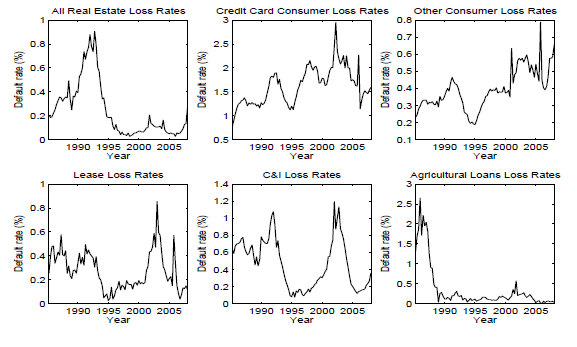
\includegraphics{figure/ch1.png}
\caption{Calibration Loan Loss Series}
\end{figure}
変換された損失率が自己回帰的である場合には、単に遅れた$\theta_t$と定数を回帰することによってこれを拡張することは容易である。 \eqref{eq:eq25}は、動的分布の場合に変換損失率が従うガウス分布を示す。 ここで、変換された損失率は条件付きガウス分布であり、AR(1)の場合、無条件のデフォルト確率q、遅れたレベルに乗る因子の2乗、$\beta$、および回帰定数からの相関パラメータ$\rho$ 、回帰係数$\theta_{t-1}$および回帰残差の標準誤差を含む。
\subsection{Results}
各四半期系列の推定結果は表1に含まれている。最初の2つの行は、無条件平均および無条件の損失率の標準偏差を示す。 クレジットカード(CC)は、平均損失が1.63%という点で、他のローンカテゴリよりもはるかに低い信用度を示してる。 対照的に、例えば農業ローン(A)は、わずか0.36%の損失率しか示さない。 しかし、クレジットカードの損失率(0.39%)のボラティリティは、他のカテゴリと同様の大きさです。 これは、クレジットカードローンが他のローンタイプよりもリスクが高いことを示唆している可能性がある。しかし、以下に示すように、リスク・アット・リスクと資本によって測定されるリスクは、デフォルト確率とデフォルト相関値ρに複雑な形で依存し、ボラティリティによって単純に要約することはできまない。
\begin{table}[H]
\begin{center}
\caption{Parameter Estimations}
\begin{tabular}{|l|l|l|l|l|l|l|}\hline
 &RE  & CC & OC & L & CI & A\\\hline
\multicolumn{7}{|c|}{Series Statistics} \\\hline
Loss rate series mean (\%) & 0.25 & 1.63 & 0.39 & 0.27 & 0.47 & 0.36\\\hline
Loss rate std dev (\%) & 0.23 & 0.39 & 0.12 & 0.16 & 0.29 & 0.56\\\hline
\multicolumn{7}{|c|}{Parameter Estimates with No Autocorrelation } \\\hline
Regression residual volatility (\%) & 30.12 & 9.62 & 10.17 & 21.74 & 24.39 & 40.37\\\hline
Factor correlation ρ (\%) & 8.32 & 0.92 & 1.02 & 4.51 & 5.62 & 14.01\\\hline
Std error ρ (\%) & 1.13 & 0.13 & 0.15 & 0.64 & 0.79 & 1.79\\\hline
Unconditional default probability q (\%) & 0.25 & 1.63 & 0.39 & 0.28 & 0.48 & 0.35\\
Std error q (\%) & 0.07 & 0.09 & 0.03 & 0.05 & 0.09 & 0.12\\\hline
\multicolumn{7}{|c|}{Parameter Estimates with Autocorrelation } \\\hline
Regression residual volatility (\%) & 8.27 & 4.25 & 4.61 & 12.19 & 6.95 & 25.77\\\hline
Factor correlation ρ (\%) & 8.67 & 0.64 & 1.05 & 4.66 & 5.3 & 13.49\\\hline
Std error ρ (\%) & 6.22 & 0.2 & 0.48 & 1.59 & 3.41 & 3.3\\\hline
Unconditional default probability q (\%) & 0.27 & 1.69 & 0.44 & 0.27 & 0.41 & 0.3\\\hline
Std error q (\%) & 0.21 & 0.13 & 0.07 & 0.06 & 0.2 & 0.1\\\hline
AR(1) parameter β  (\%) & 92.8 & 71.84 & 79.97 & 69.62 & 91.37 & 57.4\\\hline
Std error β  (\%) & 5.55 & 7.85 & 8.67 & 9.86 & 5.71 & 10.22\\\hline
\end{tabular}
\end{center}
\end{table}
$\Phi^{-1}(.)$(標準的な標準cdfの逆数)を適用することによって損失率系列に変換すると、推定回帰残差の標準偏差であるクレジットカード変換ロス率ボラティリティは、他の系列の損失率ボラティリティ 。 これは、クレジットカードの相関パラメータが0.92%に低下し、農業部門では14.01%、不動産部門では8.32%(RE)となった。 その他のコンシューマーローン(OC)の相関パラメータは1.02%であり、コーポレートおよびインダストリアルローン(CL)およびリース(L)(どちらも主にコーポレート)は5.62%および4.51%の相関パラメータを有する。\\
表1の下段には、自己相関を含むモデルの結果が報告されている。 自己相関を導入することは、変換された損失率残差の標準誤差を実質的に減少させる。 たとえば、不動産ローンの場合は30.12%から8.27%に低下する。 これは、追加の回帰因子のコンディショニング、遅れた損失、シリーズの残留揮発性が低下することが予想される。 おそらく驚くべきことに、損失率の変動性を反映しているので、相関パラメータ$\rho$は、自己相関のないモデルのものと広く匹敵する。 しかし、これは、損失率のリスク特性がシリーズが現在の平均復帰と同じであることを意味するものではない。
\section{Factors and Correlations}
\subsection{Specification Tests}
変換された各損失率の時系列から、
\begin{equation}
\tilde{\theta}_t=\frac{\Phi^{-1}(q)-\sqrt{\rho}X_t}{\sqrt{1-\rho}}
\end{equation}
この式を用いて各期間における基礎となる因子の値を推測する。 各ローンカテゴリの静的および自己相関モデルを駆動する要因を計算します。 自己相関の場合では、実際に我々が推論する共通の要素のイノベーションである。
\begin{equation}
\eta_k=\frac{X_t-\sqrt{\beta}X_{t-1}}{1-\beta}
\end{equation}
図2は、時間の経過に伴う要素の革新を示している。 自己相関モデルが正しければ、一次遅れはデータからすべての時間依存性を除去し、ショックはホワイトノイズに従うべきである。 検査では、リースおよび農業ローンにショックのクラスタリングがあり、クレジットカード債権の高次自己相関がある可能性があることが示唆されている。
\begin{figure}[H]
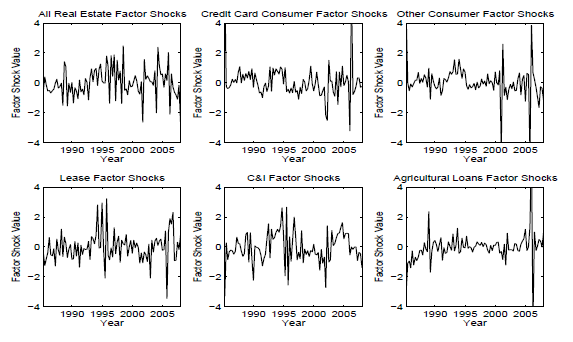
\includegraphics{figure/ch2.png}
\caption{Autoregresive Factor Shocks}
\end{figure}
\eqref{eq:eq24}における変換されたローン損失プロセスの仕様をテストするために、回帰残差のDurbin-Watsonテスト統計を計算した。 Durbin-Watson統計は、回帰の残差における自己相関をテストする。 表2は、すべてのローンロス系列のテスト統計を示している。 いずれの場合も自己相関が95%の信頼限界で残差に存在することを拒否することができ、これは要素の革新が実際に独立していることを示唆している。\\
追加のテストとして、Jarque-Beraテストを実装するという点で、さまざまなモデル(表2参照)の革新についての正規性テストを実行する。 これは、サンプルの歪度と尖度が、正規性の値から統計的に有意な程度に異なるかどうかを評価する。 漸近的に有効な信頼水準を使用するのではなく、Monte Carlosを使用してJarque-Bera検定の信頼水準を生成する。 正常性を拒否するモンテカルロの信頼水準は5.99である。\\
Durbin-WatsonとJarque-Bera検定では、残差が無相関でガウス分布であるという帰無仮説は否定されなかった。
\begin{table}[H]
\centering
\caption{Hypothesis Testing on the Autoregressive Shocks}
\begin{tabular}{|l|l|l|l|l|l|}
\hline
RE                 & CC   & OC   & L    & CI   & A    \\ \hline
Durbin-Watson 2.29 & 2.34 & 2.57 & 2.23 & 1.89 & 2.54 \\ \hline
Jarques-Bera 5.23  & 4.94 & 4.66 & 5    & 4.91 & 5.13 \\ \hline
\end{tabular}
\end{table}
\subsection{Factor Correlations}
異なるカテゴリーのローン・ロスがどのように相関しているかを調べることは興味深い。 これは、ローン市場の様々なセクター間で多様化することが、銀行がリスクを軽減するのに役立つであろう程度を明らかにすることができる。 このような疑問を尋ねるにあたり、当社の分析は、オペレーショナル・リスク、市場リスク、信用リスクなどの幅広いカテゴリーの銀行リスクの相関の程度を考慮するRosenberg and Schuermann(2006)の分析と同等である。
\begin{table}[H]
\centering
\caption{Loss Rate Correlation Matrices}
\begin{tabular}{|l|l|l|l|l|l|l|}
\hline
     & RE      & CC      & OC      & L       & CI      & A       \\ \hline
\multicolumn{7}{|l|}{Correlation Matrix with No Autocorrelation} \\ \hline
RE   & 1       & -0.4    & -0.33   & 0.37    & 0.61    & 0.37    \\ \hline
CC   & -0.4    & 1       & 0.66    & 0.2     & 0.06    & -0.33   \\ \hline
OC   & -0.33   & 0.66    & 1       & 0.38    & 0.22    & -0.23   \\ \hline
L    & 0.37    & 0.2     & 0.38    & 1       & 0.79    & 0.41    \\ \hline
CI   & 0.61    & 0.06    & 0.22    & 0.79    & 1       & 0.55    \\ \hline
A    & 0.37    & -0.33   & -0.23   & 0.41    & 0.55    & 1       \\ \hline
\multicolumn{7}{|l|}{Correlation Matrix with Autocorrelation}    \\ \hline
RE   & 1       & -0.18   & 0.11    & 0.16    & 0.28    & 0.4     \\ \hline
CC   & -0.18   & 1       & 0.26    & 0.1     & -0.1    & -0.57   \\ \hline
OC   & 0.11    & 0.26    & 1       & 0.29    & 0.06    & 0       \\ \hline
L    & 0.16    & 0.1     & 0.29    & 1       & -0.07   & 0.04    \\ \hline
CI   & 0.28    & -0.1    & 0.06    & -0.07   & 1       & 0.11    \\ \hline
A    & 0.4     & -0.57   & 0       & 0.04    & 0.11    & 1       \\ \hline
\end{tabular}
\end{table}
表3は(i)静的モデル因子系列と(ii)動的モデルからの因子革新の相関行列を、四半期データに基づく両方の場合に報告する。 自己相関のない静的モデルの相関行列は、妥当と思われる。\\
相関のパターンは、クレジットカードの損失が他の消費者ローンと最も高い相関関係を持つという点で合理的である。 すべての不動産は、ほとんどのカテゴリとかなり高い相関がある。 コーポレートローンカテゴリーであるリース、C&I、農業は、かなり高い相関がある。\\
農業ローンと不動産およびクレジットカードローンとの相関を除いて、相関の大きさは一般に動的モデルでのものより低い。 これは、静的モデルにおけるショックは、真のイノベーションの加重和と考えることができるという事実を反映している。 これらは、イノベーション自体よりもセクター間でより相関があり、無条件かつ条件付きのリスクが非常に異なるという点を強調している。\\
相関のパターンをさらに分析するために、自己相関ありと自己相関なしの2つのケースで、四半期相関行列を主成分に分解する(表4参照)。 相関行列が1つまたは2つの因子を有する因子から、多くの因子までの相関行列からどれだけ離れているかを分析するために、最大の固有値の大きさを調べることができる。 また、ローン・ロス・カテゴリのどれが異なる要因によって駆動されるように見えるかもしれない。\\
まず、相関行列の固有値の大きさを評価する仮説検定を行った。 これは個々の貸倒率を動かす要因に経済的に重要な共通要因がいくつあるかを明らかにしている。 簡単に言えば、統計は、特定の信頼水準で、異なる固有値に関連する主成分が共通の変動性の相当量をもたらすかどうかをテストする。\\
まず、固有値が昇順に並べられ、 最小のp個の固有値が合計され、合計が無視できるという仮説に対してそれらの合計がテストされる。表5は、様々な信頼レベルで仮説を棄却する固有値の数を示している。 テストでは、静的モデルと動的モデルの両方で、複数の主成分がローンロス系列間の相関に重要な役割を果たすことが示唆されている。\\
表4を見ると、小売タイプのカテゴリー、クレジットカードおよびその他の消費者は、最も重要な因子に負の相関を示し、次の最も重要な因子については正の相関を示す因子に同じ符号が付いていることに気付くことがある。 コーポレート・ローンカテゴリー、C&Iおよびリースは、主にこれらの要因にプラスのウェイトをもたせている(マイナスの小さな動的ケースのリースを除く)。 最大の要素は、ビジネスセクター間で差別化していると見なすことができますが、次はビジネスサイクル効果のほうが大きくなる可能性がある。
\begin{table}[H]
\centering
\caption{Principal Component Analysis of Factor Correlations}
\begin{tabular}{|l|l|l|l|l|l|l|l|}
\hline
                & Eigenvalue & RE    & CC    & OC    & L     & CI    & A     \\ \hline
\multicolumn{8}{|l|}{Eigenvalue and Factor Weights with No Autocorrelation}  \\ \hline
Common Factor 1 & 0.11       & 1.42  & 0.43  & 0.77  & 0.57  & -2.25 & 0.9   \\ \hline
Common Factor 2 & 0.23       & 0.54  & 0.03  & 1.01  & -1.59 & 0.51  & 0.55  \\ \hline
Common Factor 3 & 0.34       & -0.25 & -1.33 & 0.94  & 0.34  & -0.13 & -0.3  \\ \hline
Common Factor 4 & 0.64       & 0.8   & 0.04  & -0.01 & -0.02 & 0.13  & -0.95 \\ \hline
Common Factor 5 & 2.08       & -0.16 & 0.41  & 0.44  & 0.24  & 0.15  & -0.11 \\ \hline
Common Factor 6 & 2.6        & 0.29  & -0.09 & -0.02 & 0.3   & 0.35  & 0.28  \\ \hline
\multicolumn{8}{|l|}{Eigenvalue and Factor Weights with Autocorrelation}     \\ \hline
Common Factor 1 & 0.41       & 0.61  & -0.76 & 0.33  & -0.14 & -0.26 & -1.15 \\ \hline
Common Factor 2 & 0.66       & 0.74  & 0.46  & -0.02 & -0.64 & -0.53 & 0.28  \\ \hline
Common Factor 3 & 0.75       & 0.49  & 0.22  & -0.78 & 0.64  & 0.03  & -0.2  \\ \hline
Common Factor 4 & 1.13       & -0.15 & -0.2  & 0.12  & 0.42  & -0.77 & 0.21  \\ \hline
Common Factor 5 & 1.61       & 0.34  & 0.14  & 0.53  & 0.37  & 0.21  & 0.15  \\ \hline
Common Factor 6 & 2.3        & 0.21  & -0.47 & -0.13 & -0.04 & 0.13  & 0.36  \\ \hline
\end{tabular}
\end{table}
\section{Conditional Default Rate Distribution}
\subsection{Conditioning  on  Macroeconomic Variables}
銀行のポートフォリオのリスク分析は、通常、将来のポートフォリオ価値の分布に関するVaRやExpected Shortfallsなどの統計を計算することによって実行される。これらの統計は、一般的に、無条件で計算される。つまり、将来発生する可能性のあるイベントを条件とすることはない。\\
しかし、条件付きリスク統計を検討することも興味深い。 景気後退の場合にポートフォリオがどのように挙動するかを評価したいと思うかもしれない(失業や生産高のようなマクロ経済変数の所与の悪化によって測定される)。 そのような分析は、しばしばストレステストと呼ばれる。 ストレステスト方法論の研究には、Kupiec(1998)、Berkowitz(1999)、Longin(2000)、Peura and Jokivuolle(2004)が含まれる。 最近の不履行確率に関する実証研究では、Pesaran、Schuermann、Treutler、Weiner(2006)、Pesaran、Schuermann、Weiner(2004)は、ローン債券ポートフォリオのリスク分析をマクロ経済ショックに条件付けると考えている、 クレジットポートフォリオのストレステスト方法がある。
\begin{table}[H]
\centering
\caption{Hypothesis Testing of Eigenvalues}
\label{my-label}
\begin{tabular}{|l|l|l|l|l|}
\hline
Confidence Limit              & 75\% & 85\% & 90\% & 95\% \\ \hline
Model with No Autocorrelation & 4    & 3    & 3    & 2    \\ \hline
Model with Autocorrelation    & 3    & 2    & 1    & 1    \\ \hline
\end{tabular}
\end{table}
観察可能なマクロ経済要因と観察不能な共通要因の組み合わせによってデフォルト率を引き上げるこのセクションで開発したアプローチは、債務不履行と債務不履行確率を調査するためのハザード・アプローチを用いた序論に要約されている最近の研究に関連している。 特に、Duffie、Saita、Wang(2007)は、観察可能な変数の変動がデフォルト確率間の相関を引き起こすと仮定している。 Das、Duffie、Kapadia、Saita(2007)は、観察可能な運転変数を持つハザードによって生成されたデフォルトが予想以上に相関しているかどうかを調べる。 Duffie、Eckner、Horel、Saita(2006)は、観察された運転プロセスと観察されない運転プロセスの組み合わせでハザードモデルを推定する方法を示している。\\
このセクションでは、ローン・ロス・分布が、ストレス・シナリオの枠組みと分析に適した条件付きの条件でどのように表現されるかを考察する。 債務者iは、式(1)に基づいて時刻tにおいてデフォルトと仮定されることを想起されたい。 ここで、潜在的な確率変数$Z_{i,t}$が、観測された要因と観察されない要因の合計から構成されているものとする。
\begin{equation}
Z_{i,t}=\sqrt{\rho}\bigl(\sqrt{1-\lambda^2} X_t +
\lambda \sum_{j=1}^J a_j^{\star} Y_{j,t} \bigr)+\sqrt{1-\rho}\epsilon_{i,t}.
\end{equation}
$Y_{j,t}$は観測可能なマクロ経済変数であると仮定する。 これらの変数について条件を定めるので、これらの変数がどのようなプロセスに従うかを正確に指定する必要はない。$X_{i,t}$は以前のような一次自己回帰的確率過程であり、$S_{i,t},\eta_t$は独立した標準正規分布であると仮定される。$\lambda$は、観測されたおよび観測されない因子の$Z_{i,t}$への寄与を決定する。$\lambda\in(0,1)$とする。\\
無条件に、$Zi_t$に単位分散があることを保証するために、観測可能な因子の重みを次のように再定義することによって.$\sum_{i=1}^{J}a_j^{\star}Y_{j,t}$、項を再スケーリングする。
\begin{equation}
a_j = \frac{a_j^{\star}}{\sqrt{\Sigma_{k=1}^{J}\Sigma_{m=1}^{J} a_k a_m Cov(Y_{k,i},Y_{m,i})}}
\end{equation}
債務者iのデフォルトドライバを以下のように修正する。
\begin{equation}
Z_{i,t}=\sqrt{\rho}\bigr(\sqrt{1-\lambda^2}X_t + \lambda a'Y\bigl)+\sqrt{1-\rho}\epsilon_{i,t}
\end{equation}
ここで、$\sum a_j Y_j$は、因子とその重みがベクトルとして表現されるという点で抑制されている。 $Y_{j,t}$は定常系列と仮定されるので、共分散行列は時間とは無関係である。\\
マクロ・コノミック要因に基づく損失率条件付きの動的過程の導出は、第2節のそれに密接に従う。$X_{t-1}$およびYに関する条件付き損失率分布は、
\begin{equation}
W(\theta_t)\equiv\Phi(\frac{\sqrt{1-\rho}\Phi^{-1}(q)+\sqrt{\rho}\sqrt{1-\lambda^2}\sqrt{\beta}X_{t-1} + \sqrt{\rho}\lambda aY }{\sqrt{\rho}\sqrt{1-\lambda^2}\sqrt{1-\beta}})
\end{equation}
従って、変換損失率$\theta_t\equiv\Phi^{-1}(\theta_t)$は、以下のガウス分布に従う。
\begin{equation}
N\Bigl(\frac{\Phi^{-1}(q)-\sqrt{\rho}\sqrt{1-\lambda^2}\sqrt{\beta}X_{t-1}-\sqrt{\rho}\lambda aY}{\sqrt{1-\rho}},\frac{\rho(1-\lambda^2)(1-\beta)}{1-\rho} \Bigr)
\end{equation}
このことから、変換された損失率は、その平均、標準偏差およびショックの観点から表現される。 次に、これを再構成し、遅らせ、式(2)に代入して、観測可能な確率論的プロセスに条件付きの変換損失率の自己回帰プロセスを導出することができる。\\
{\bf 命題3}\\
個々の借り手の潜在変数$Z_{i,t}$と、観測されていない共通因子$X_t$は、貸出数$n\rightarrow\infty$とすると、式(35)、(5)の処理に従い、変換損失率$\tilde{\theta}_t\equiv\Phi^{-1}(\theta_t)$は次のように収束する
\begin{eqnarray}
\tilde{\theta}_t&=&\sqrt{\beta}\tilde{\theta}_{t-1}+\frac{1-\sqrt{\beta}}{\sqrt{1-\rho}}\Phi^{-1}(q)\\
&&-\frac{\sqrt{\rho}}{\sqrt{1-\rho}}\lambda a(Y_t-\sqrt{\beta}Y_{t-1})-\frac{\sqrt{\rho}\sqrt{1-\lambda^2}}{\sqrt{1-\rho}}\sqrt{1-\beta}\eta_t
\end{eqnarray}
\subsection{Estimation}
先に説明した2つの損失率系列、すなわちクレジットカード損失とC&I損失を使用して、上記のモデルを実装する。 これまでのように、シリーズは、バーゼル銀行監督委員会(1999年)に含まれるLGDの見積りによって再スケーリングされた。\\
多因子ストレスを作成し、結果を明確にするために観察されたいくつかのマクロ変数を調整することは、我々の枠組みにおいては単純であるが、我々は単変量および二変量の症例に限定する。 具体的には、米国の雇用率と米国の工業生産を含むストレスを考慮する。これらのシリーズは、米国労働省と米国連邦準備制度のそれぞれから来ており、いずれの場合も毎月利用可能である。 これらの系列のレベルの時系列プロットが図3に示されている。
\begin{figure}[H]
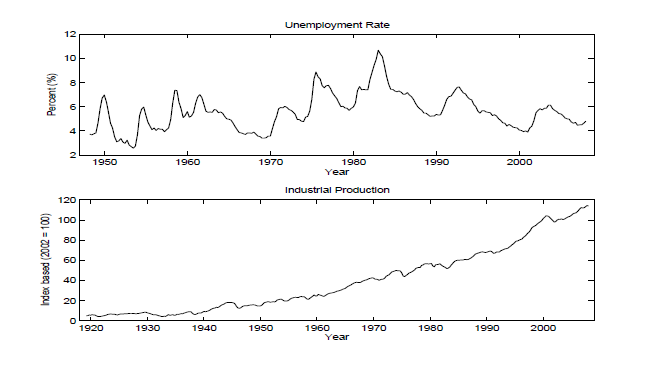
\includegraphics{figure/ch3.png}
\caption{Macro-Economic Stress Parameters}
\end{figure}
デフォルト率は失業率の変化と生産の伸びに影響を受けると予想するのがより妥当と思われたので、我々は過去12ヶ月間の変化率として2つの系列を表現した。 我々はサンプルの標準偏差で割ることによって系列を正規化した。 図4は、ストレス推定に用いられる正規化された系列を示す。
\begin{figure}[H]
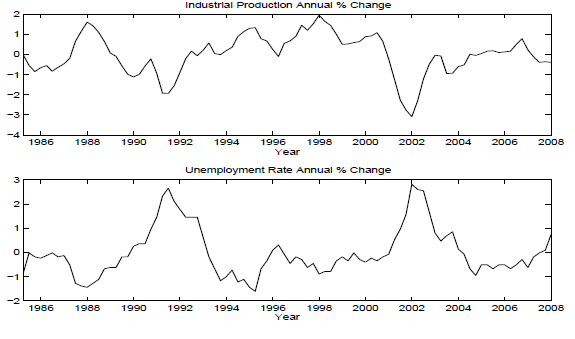
\includegraphics{figure/ch4.png}
\caption{Normalised Stress Series}
\end{figure}
条件付きデフォルト分布のパラメータを推定するために、再び最尤法を使用した。 多変量設定では、観測された応力係数の重みは、$Z_{i,ts}$が単位分散を持つように正規化されなければならない。
\subsection{Stress Estimates}
ここでは、(i)米国失業率の年率変化率を条件とするクレジットカード損失率、(ii)同じマクロ経済変数を条件とするC&I損失率の2つの単変量ストレスを報告する。 表6は、2つのケースにおけるモデルのパラメータ推定値を示す。
\begin{table}[H]
\centering
\caption{Univariate Stress Parameterisation}
\begin{tabular}{|l|l|l|l|l|}
\hline
                                                                                     & \multicolumn{2}{l|}{CC} & \multicolumn{2}{l|}{CI} \\ \hline
\begin{tabular}[c]{@{}l@{}}Factor correlation ρ\\   (\%)\end{tabular}                & 0.6       & (-3.83)     & 4.24      & (-1.87)     \\ \hline
\begin{tabular}[c]{@{}l@{}}Unconditional default\\   probability q (\%)\end{tabular} & 1.67      & (-16.15)    & 0.38      & (-2.75)     \\ \hline
AR(1) parameter β  (\%)                                                              & 68.14     & (-8.32)     & 89.58     & (-14.57)    \\ \hline
\begin{tabular}[c]{@{}l@{}}Stress coefficient λ\\   (\%)\end{tabular}                & -37.56    & (-2.88)     & -26.22    & (-2.34)     \\ \hline
\end{tabular}
\end{table}
クレジットカード損失の場合、因数相関$\rho$は0.60%である。 無条件のデフォルト確率$\rho$は1.67%とかなり高く、観察不能因子の復帰パラメータ$\beta$は68.14%である。 応力係数$\lambda$は-37.56%である。 ストレス係数の符号は正しい。 応力係数は負である。 これは、失業率が上昇するにつれて、$Z_{its}$が減少し、デフォルト数が直感的に増加することを意味する。\\
C\&I損失パラメータはわずかに異なる。 因子相関$\rho$は、4.24%のクレジットカードよりもはるかに大きい。 無条件のデフォルト確率qは0.38%ではるかに低く、係数の逆転率は89.58%で高い。 再び、ストレス係数は正しい負の符号を持つので、失業率に対するコンディショニングの影響が期待される効果を有する。\\
表1を見ると、これらの結果を動的モデルの元の推定と比較できる。 パラメータ推定値はすべてわずかに小さい。 相関とデフォルトの確率はどちらも低い。 したがって、観察された因子にコンディショニングを行うことにより、モデルにおけるランダム性またはリスクが低減される。\\
多変量ストレスの例として、(a)米国の失業率の年次変化と(b)米国の工業生産における年率の変化に対するC&I損失率を考慮した。 表7は、このストレスの場合のモデルパラメータの推定値を示す。\\
これらの結果を元の推定値および単変量ストレスと比較すると、やはりパラメータが減少しているか類似している。 相関は4.24%から4.18%に低下し、無条件のデフォルト確率は同じである。 したがって、再び観察可能な要因を強調することによって、システムのリスクが低下した。\\
したがって、景気後退または同様の周期的事象を記述するマクロ経済変数の賢明な選択によって、これらの変数を調整し、リスクの影響を評価することができる。 次のセクションでは、これらのアイデアについてさらに説明する。
\begin{table}[H]
\centering
\caption{Multivariate Stress Parameterisation}
\begin{tabular}{|l|l|l|}
\hline
                                                                                        & \multicolumn{2}{l|}{CI} \\ \hline
\begin{tabular}[c]{@{}l@{}}Factor correlation ρ\\   (\%)\end{tabular}                   & 4.18      & (-1.94)     \\ \hline
\begin{tabular}[c]{@{}l@{}}Unconditional default\\   probability q (\%)\end{tabular}    & 0.38      & (-3.01)     \\ \hline
AR(1) parameter β  (\%)                                                                 & 89.38     & (-14.99)    \\ \hline
\begin{tabular}[c]{@{}l@{}}Unemployment\\   coefficient auλ (\%)\end{tabular}           & -23.18    & (-1.92)     \\ \hline
\begin{tabular}[c]{@{}l@{}}Industrial production\\   coefficient aipλ (\%)\end{tabular} & 5.37      & (-0.56)     \\ \hline
\end{tabular}
\end{table}
\subsection{Stressed Default Rate Distributions}
特定のマクロ経済シナリオを調整することにより、変化した損失率の分布がどのように影響を受けるかを調べるために、4年間の損失率のモンテカルロシミュレーションを実施した。 我々は、米国失業率データが入手可能であるサンプル期間に観察された4年間の失業率の年率差の最大の正の変化を条件付けたという極端な期間を選択した。 これは1950-1954年の期間であり、図5はこの年の失業率を示している。
\begin{figure}[H]
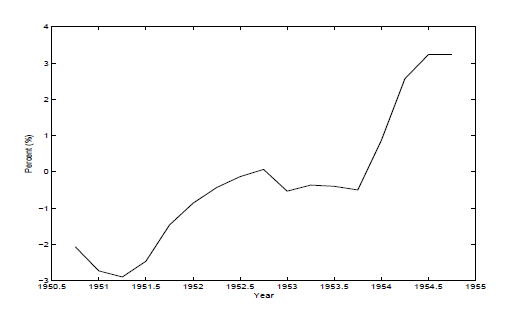
\includegraphics{figure/ch5.png}
\caption{Unemployment Recession Stress}
\end{figure}
\begin{figure}[H]
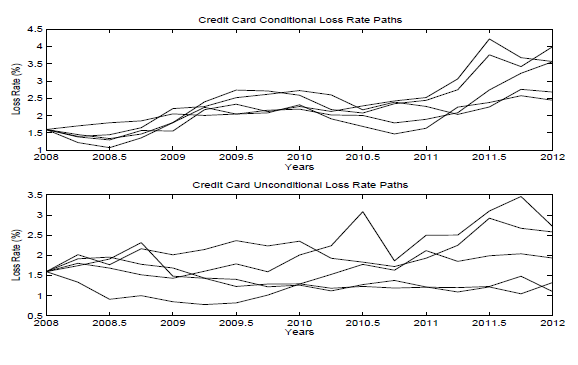
\includegraphics{figure/ch6.png}
\caption{Stress Monte Carlo Paths}
\end{figure}
図6は、条件付きおよび無条件のケースで4年間にわたってシミュレートされたクレジットカード損失率を示している。 これらの損失経路の形状を失業率ストレスと比較すると、図5では、損失率が観察可能な要因によってどのように推移するかを見ることができる。 期間4の損失は、無条件の場合と比較して平均して劇的に増加している。\\
図7は、1年および4年の視野におけるシミュレーションされた損失分布を示している。表8は、これらの分布の統計を示している。最初の4年間を見ると、失業ストレスがクレジットカードの損失率をどのように上昇させたかがわかる。平均損失は現在3.19%だが、無条件の場合は1.69%である。\\
1年間の地平線の損失率は、異なる画像を提示する。 図5において、失業率は実際には最初の年の中間に低下し、その後再び上昇して開始時の値よりもわずかに上回ることに注意する。 1年間で失業率が上昇したため、条件付きケースの平均損失は無条件ケースより1.81%高く、1.69%となった。 しかし、上半期の失業率の低下により、これは損失分配のボラティリティを減少させる。
\section{Capital Implications}
\subsection{Implied Capital}
このセクションでは、資本モデリングの動的デフォルト率の影響を考慮する。 期間tにおける銀行のポートフォリオにおける損失が、上記の単一のリスク要因、すなわち$X_t$の関数であると仮定する。 Gordy(2003)に示されているように、単一ローンのマージナル・バリュー・アット・リスク(MVaR$\alpha$)は、エクスポージャーのエクスポージャーの期待損失として、$X_t$がその$\alpha$-分位数であるとして計算することができる。 しかし、予想される損失はデフォルトの確率$\Phi(\tilde{\theta})$に既定の損失(LGD)を掛けたもの、すなわち、
\begin{equation}
MVaR_{\alpha} = LGD \times \Phi(\frac{\Phi^{-1}(q)-\sqrt{\rho}\sqrt{\beta}X_{t-1}-\sqrt{\rho}\sqrt{1-\beta}\Phi^{-1}(\alpha)}{\sqrt{1-\rho}})
\end{equation}
ここで、因子ショック$\eta_t$は、その$\alpha$-分位数で取られる。
t-1における情報上のデフォルト条件付き確率は、式(9)によって与えられる。 代入すると命題が得られる\\
{\bf 命題4}\\
上記の仮定の下で、MVaRαと表示された単一ローンのリスク・アット・リスク・アット・リスクは、
\begin{equation}
MVaR_\alpha = LGD \times \Phi(\sqrt{1-\rho\beta}\frac{\Phi^{-1}(q_t)-\sqrt{\rho}\sqrt{1-\beta}\Phi^{-1}(\alpha)}{\sqrt{1-\rho}})
\end{equation}
バーゼルIIの資本式は、予期せぬ損失、すなわちMVaRαから予想損失
\begin{equation}
Basel Capital Formula = LGD \times \Phi(\frac{\Phi^{-1}(q) + \sqrt{\rho}\sqrt{1-\beta}\Phi(\alpha^{\star})}{\sqrt{1-\rho}})-LGD\times q
\end{equation}
ここで、$\alpha^{\star}$は$1-\alpha$に等しい。 ここで、バーゼル式は、式$\sqrt{1-\rho\beta}$が存在しないことによって単純化され、条件付きデフォルト確率qtではなくqに依存することに注意する。
因子がもはや自己相関しないように$\beta=0$である場合、後者の項はすべてのtに対して一に単純化し、$q_t=q$に単純化する。 この場合、$\phi-1(\alpha^{\star})=-\phi-1(\alpha)$であるから、バーゼル資本の数式は、式(42)のMVaRαの式に等しい。
\begin{figure}[H]
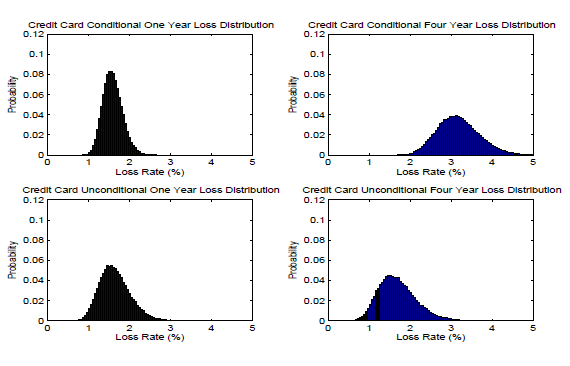
\includegraphics{figure/ch7.png}
\caption{Calibration Loan Loss Series}
\end{figure}
\subsection{Stressed Loss Distributions}
データ期間が1年の場合、規制当局と銀行が使用する資本料金を関連付けるのは簡単な練習である。 したがって、四半期ごとのデータを以下の資本計算のための年次表記に変換する。\\
我々はバーゼルⅡの規則の下で自己資本の有無にかかわらず、推定プロセスによって暗示されたMVaRに基づいて資本を計算する。 バーゼルIIの計算では、ポイントインタイムのデフォルト確率がその式のパラメータとして仮定される。 このパラメータのサンプル期間の終わりに損失率を取る。これは、条件付きデフォルト確率のプロキシとみなすことができるからである。\\
表9は、すべてのモデルによって計算された資本要件を報告している。 表の上半分には、バーゼルⅡ計算で想定されるパラメータが表示される。 表の下半分は、3つの異なるケースの資本を報告する。 自己相関の場合に暗示される資本は、すべての系列の静的な場合よりも小さいことがすぐに分かる。 不動産カテゴリの場合、自己相関の場合の暗黙の資本は0.61%であり、これは2.35%の静的な場合の約5倍である。 しかし、他のシリーズは、相対的には近い。 クレジットカード計算は、条件付きデフォルト確率の代理人と見ることができるので、静的ケースでは3.87%、自己相関ケースでは2.16%を意味する。\\
バーゼルⅡの資本比較はさらに顕著である。 自己相関の有無に関わらず、暗示された資本は、バーゼルが提示しているものよりも実質的に少ない。 一例として、他の消費者カテゴリーは、自己相関モデルを用いて1.11%、静的モデルで2.09%、バーゼルIIルールで8.26%を意味する。 すべての場合において、バーゼルⅡの計算では、自己相関モデルより少なくとも4倍以上の大きさがあり、場合によってはさらに大きくなる。\\
このような場合のバーゼルパラメータ設定は、Creditmetricsなどの格付けベースのモデルによる経済損失モードのMVaRに基づいているため、不動産、リース、C&Iなどの長期性資産の場合は驚くべきことではある。 (デフォルトモードの資本曲線式は、都合のよい便利な機能ですが、小売り(特にクレジットカード)を含む短期資産の場合、この暗黙の資本金の差は、銀行や金融機関にとって非常に重要とみなされる。 \\
本稿では、広く使われているVasicekの貸倒損失モデルの一般化を示す。 私たちの一般化は、ローン・ロス・ディストリビューションのダイナミックな進化を可能にする。ローンロスが自己相関と傾向の明確な兆候を示しているため、このモデルを実生活データの分析に使用するには、ダイナミクスの導入が不可欠である。
分析では、集約レベルでのポートフォリオの信用リスクを調べるためのフレームワークと一連のツールが提供される。結果は、条件付きおよび無条件の世界における損失特性のリスク特性および損失の一般的な挙動が非常に異なることを示している。
\begin{table}[H]
\centering
\caption{Stressed Loss Distribution Statistics}
\begin{tabular}{|l|l|l|l|l|}
\hline
              & \multicolumn{2}{l|}{Conditional} & \multicolumn{2}{l|}{Unconditional} \\ \hline
              & Year 1          & Year 4         & Year 1           & Year 4          \\ \hline
Mean          & 1.81            & 3.19           & 1.66             & 1.69            \\ \hline
Median        & 1.79            & 3.15           & 1.62             & 1.64            \\ \hline
90\% quantile & 2.19            & 3.86           & 2.2              & 2.3             \\ \hline
95\% quantile & 2.31            & 4.09           & 2.39             & 2.53            \\ \hline
\end{tabular}
\end{table}
\section{Conclusion}
本稿では、広く使われているVasicekの貸倒損失モデルの一般化を示す。我々の一般化は、ローン・ロス分布のダイナミックな進化を可能にする。ローンロスが自己相関と傾向の明確な兆候を示しているため、このモデルを実生活データの分析に使用するには、ダイナミクスの導入が不可欠である。\\
この分析では、集約レベルでのポートフォリオの信用リスクを調べるためのフレームワークと一連のツールが提供されている。結果は、条件付きおよび無条件の世界における損失特性のリスク特性および損失の一般的な挙動が非常に異なることを示している。\\
マクロ経済変数や指標にモデルをリンクすることは、このモデルを使用する単純な作業である。
これは、銀行や他の金融機関がダイナミックな意味でリスクを分析し、ビジネスサイクル効果のストレステストを可能にするのに役立つ。
\begin{table}[H]
\centering
\caption{Capital Calculations}
\begin{tabular}{|l|l|l|l|l|l|l|}
\hline
                              & RE         & CC        & OC        & L         & CI        & A         \\ \hline
\multicolumn{7}{|l|}{Common  Parameters}                                                               \\ \hline
Default probability (\%)      & 0.63       & 5.95      & 2.37      & 0.53      & 1.08      & 0.21      \\ \hline
Loss given default LGD        & 0.35       & 0.65      & 0.65      & 0.45      & 0.45      & 0.45      \\ \hline
\multicolumn{7}{|l|}{\begin{tabular}[c]{@{}l@{}}Factor Correlation Estimates ρ \\   (\%)\end{tabular}} \\ \hline
Basel II                      & 15         & 4         & 8.66      & 21.22     & 19        & 22.83     \\ \hline
With no autocorrelation       & 10.53      & 1.31      & 1.33      & 5.16      & 7.25      & 13.98     \\ \hline
With autocorrelation          & 10.91      & 0.88      & 1.43      & 5.22      & 7.17      & 6.84      \\ \hline
AR(1) parameter β  (\%)       & 80.07      & 44.82     & 66.68     & 41.33     & 65.03     & 59.15     \\ \hline
\multicolumn{7}{|l|}{Capital Calculations (\%)}                                                        \\ \hline
Basel II                      & 3.37       & 7.97      & 8.26      & 5.7       & 7.59      & 3.56      \\ \hline
With no autocorrelation       & 2.35       & 3.87      & 2.09      & 1.38      & 3         & 1.98      \\ \hline
With autocorrelation          & 0.61       & 2.16      & 1.11      & 0.89      & 1.28      & 0.42      \\ \hline
\end{tabular}
\end{table}
\end{document}

